
\section{Nền tảng iOS và các thành phần cơ bản}
    \subsection{Kiến trúc tầng của iOS}
        \begin{flushleft}
            \begin{figure}[H] % hoặc [h], [t], [b] tùy vị trí
                \centering
                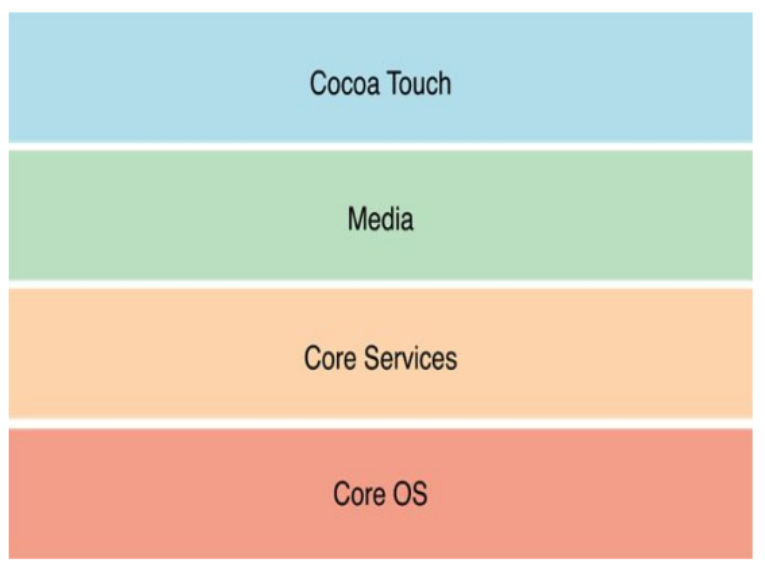
\includegraphics[width=0.8\textwidth]{images/kientrucios.png}
                \caption{Kiến trúc phân tầng IOS}
                \label{fig:kientrucios}
            \end{figure}

        IOS có kiến trúc nhiều tầng, mỗi tầng cung cấp các framework và dịch vụ khác nhau:\\
            \textbf{Cocoa Touch:} Tầng cao nhất, cung cấp cáp framework cốt lõi như UIKit và SwiftUI cho phát triển giao diện người dùng.\\
            \textbf{Media:} Chứa các công nghệ đồ họa, âm thanh và video như Core Graphics, Core Animation, AVFoundation.\\
            \textbf{Core Services:} Cung cấp các dịch vụ cơ bản như Core Data, Core Location, và Foundation framework.\\
            \textbf{Core OS:} Tầng thấp nhất, bao gồm kernel, file system, bảo mật, và các dịch vụ hệ thống cấp thấp.\\
       
        \end{flushleft}
   \subsection{ Vòng đời ứng dụng IOS}	
        \begin{flushleft}
            Khi user mở điện thoại của mình lên thì không có ứng dụng nào chạy cả ngoài những thứ nằm trong Operation system . Application của bạn cũng sẽ không chạy. Sau khi user nhấn vào icon của app, Springboard sẽ kích hoạt application của bạn. Application cùng với các thư viện của nó sẽ được thực thi và được tải vào bộ nhớ, trong khi đó thì Springboard sẽ nhận nhiệm vụ hiển thị màn hình launch screen của ứng dụng. Sau cùng thì ứng dụng của bạn bắt đầu được chạy và application delegate sẽ nhận được các notification.
Các iOS app chạy trên các thiết bị đều có các trạng thái chuyển đổi như: Not running, In active, Active, Background, Suspended. Tại bất kì thời điểm nào, app của bạn đều rơi vào các trạng thái trên.
        \end{flushleft}
        \begin{figure}[H] % hoặc [h], [t], [b] tùy vị trí
            \centering
            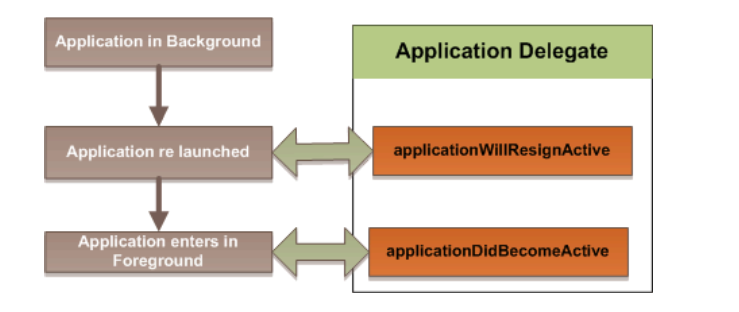
\includegraphics[width=0.8\textwidth]{images/vongdoiios.png}
             \caption{Vòng đời ứng dụng IOS}
            \label{fig:vongdoiios}
        \end{figure}
         \begin{flushleft}
            \textbf{NotRunning:}Ứng dụng chưa được khởi chạy hoặc đã bị hệ thống chấm dứt.
            \textbf{Inactive:} Ứng dụng đang chạy ở foreground nhưng không nhận events (ví dụ: khi có cuộc gọi đến).\\
            \textbf{Active:} Trạng thái bình thường khi ứng dụng chạy ở foreground và đang xử lý events.\\
            \textbf{Background:} Ứng dụng không hiển thị nhưng vẫn chạy và thực thi mã.\\
            \textbf{Suspended:} Ứng dụng ở background nhưng không chạy mã, có thể bị hệ thống chấm dứt để giải phóng tài nguyên.
         \end{flushleft}
   \subsection{App Delegate và Scene Delegate}	
         \begin{flushleft}
            \textbf{AppDelegate:} Quản lý vòng đời chung của ứng dụng và cấu hình ban đầu.
            \textbf{SceneDelegate:} Quản lý UI lifecycle của từng cửa sổ ứng dụng (scene).
         \end{flushleft}

   \subsection{Luồng làm việc của người dùng và Storyboards}
        \begin{flushleft}
            \textbf{Storyboards:} Công cụ trực quan để thiết kế và quản lý luồng màn hình trong ứng dụng.\\
            \textbf{Segues:} Xác định chuyển tiếp giữa các màn hình.\\
            \textbf{Programmatic UI:} Phương pháp thay thế để tạo UI bằng mã Swift.
        \end{flushleft}